%!TEX root = Manuscript.tex

%解释DSM,DoD,GCP,multi-epoch, intra and inter epoch, GT
\chapter{Introduction en français}
\label{chap:introFrench}
\minitoc

\section{Motivation et objectifs}
\subsection{Pourquoi les images historiques sont-elles intéressantes}
Les images aériennes historiques (c'est-à-dire analogiques ou d'archives) jouent un rôle important en fournissant des informations uniques sur l'évolution de la couverture terrestre. 
Ce sont des atouts précieux pour un grand nombre d'applications telles que (1) l'analyse des catastrophes naturelles (par exemple, tremblement de terre, glissement de terrain, volcan, inondation, avalanche, etc.), (2) la surveillance éco-environnementale (par exemple, forêt, atmosphère, glacier, eau, littoral, etc.), (3) l'expansion urbaine et (4) la pollution et la protection de l'environnement, etc.
\par
Les images aériennes historiques ont été régulièrement acquises depuis les années 1920 par des agences cartographiques, militaires ou cadastrales du monde entier. Une quantité massive d'entre elles ont été numérisées et rendues accessibles par des services web~\cite{sebastien2019archiving,earthexplorer,remonterletemps}. 
Par exemple, selon une enquête réalisée au début de 2017 en Europe~\cite{sebastien2019archiving}, il y a environ 50 millions d'images aériennes archivées en Europe, dont environ 37,8\% sont numérisées. 
Les images sont de haute résolution spatiale, et sont acquises en configuration stéréoscopique, permettant la restitution 3D des territoires. 
Elles sont souvent accompagnées de métadonnées, comprenant dans la plupart des cas la focale de la caméra, la hauteur de vol, l'échelle et la taille physique du capteur, qui sont généralement enregistrées ou mentionnées sur les films. D'autres métadonnées telles que les plans de vol, les certificats d'étalonnage de la caméra ou les orientations ne sont pas couramment disponibles. 
\par
Lorsque les paramètres d'étalonnage de la caméra sont inconnus, ils doivent être évalués au moyen d'une procédure appelée ajustement du faisceau d'auto-étalonnage. \ac{GCP}s sont nécessaires, sinon des paramètres de caméra estimés de manière inexacte entraîneront des surfaces d'erreur systématiques appelées effet de dôme (c'est-à-dire effet de bol).
En général, les \ac{GCP}s proviennent (1) de mesures sur le terrain \cite{micheletti2015application,walstra2004time,cardenal2006use}, (2) d'orthophotos et de \ac{DSM} récents \cite{nurminen2015automation,ellis2006measuring,fox2008unlocking} et (3) d'images satellites récentes \cite{ellis2006measuring,ford2013shoreline}. Le plus difficile est d'identifier les \ac{GCP}s sur les images historiques, ce qui n'est pas facile en raison des inévitables changements de scène. Les \ac{GCP} sont généralement mesurés manuellement à l'aide de photos récentes, mais cela reste monotone et laborieux. 
Il est urgent d'identifier automatiquement les points correspondants (c'est-à-dire les correspondances) sur des images historiques et récentes.\\
Lorsque les utilisateurs sont uniquement intéressés par la comparaison de différentes époques historiques, l'auto-calibrage peut être réalisé sans \ac{GCP}s. Les correspondances entre différentes époques serviraient d'observations dans l'ajustement du faisceau pour éliminer les erreurs systématiques des surfaces. En conclusion, le goulot d'étranglement de l'auto-calibration des images historiques est la récupération des correspondances sur des images prises à des époques différentes (c'est-à-dire multi-époques).



\subsection{Comment faire correspondre des images historiques multi-époques}
Cependant, la comparaison d'images historiques multi-époques reste difficile, malgré le fait qu'il existe un grand nombre d'algorithmes de comparaison d'images dont l'efficacité a été prouvée sur des images modernes. Les raisons en sont les suivantes:\\
\begin{enumerate}
	\item Les images multi-époques sont souvent acquises à différents moments de la journée et par différents temps et saisons, ce qui entraîne inévitablement des différences d'apparence.
	\item La scène change au fil du temps en raison de phénomènes anthropiques (par exemple, l'urbanisme) ou naturels (par exemple, un tremblement de terre), en particulier pour les grands écarts temporels.
	\item Les images multi-époques présentent souvent des résolutions spatiales hétérogènes, accompagnées de conditions d'acquisition différentes (capteurs, canaux spectraux, etc).
	\item Les images historiques sont souvent confrontées à une faible qualité radiométrique, notamment un faible contraste, du bruit d'image, une détérioration causée par le vieillissement des films, ou même des rayures sur les films.
\end{enumerate}
La simple application de méthodes d'appariement des caractéristiques (par exemple, SIFT~\cite{lowe2004distinctive} ou SuperGlue~\cite{sarlin2020superglue}) sur des paires d'images multi-époques donne souvent des résultats insatisfaisants. Un exemple est donné dans la Figure~\ref{MultiEpoqueImgPaire}. Une paire d'images multi-époques est représentée avec des rectangles rouges indiquant la zone de chevauchement sur la Figure~\ref{MultiEpoqueImgPaire}(a). Les images de gauche et de droite ont été prises au même endroit en 1954 et 1970 respectivement. La scène a changé de manière significative, beaucoup de nouveaux bâtiments sont apparus, les tons de couleur étaient très différents. Dans la Figure~\ref{MultiEpoqueImgPaire}(b-d), les résultats de correspondance de SIFT, SuperGlue et le nôtre sont affichés pour comparaison. Comme on peut le voir, SIFT n'a trouvé aucune correspondance. SuperGlue a trouvé 369 correspondances, dont la plupart semblent bonnes, mais en regardant plus attentivement, les détails révèlent une faible précision de localisation. Notre méthode a trouvé 1463 correspondances avec une grande précision, grâce à l'aide (1) de la géométrie 3D et (2) de la stratégie diviser et conquérir (c'est-à-dire grossier-à-précis), qui sont détaillées dans les textes suivants.
\begin{figure*}[htbp]
	\begin{center}
		\subfigure[Paire d'images multi-époques]{
			\begin{minipage}[t]{0.45\linewidth}
				\centering
				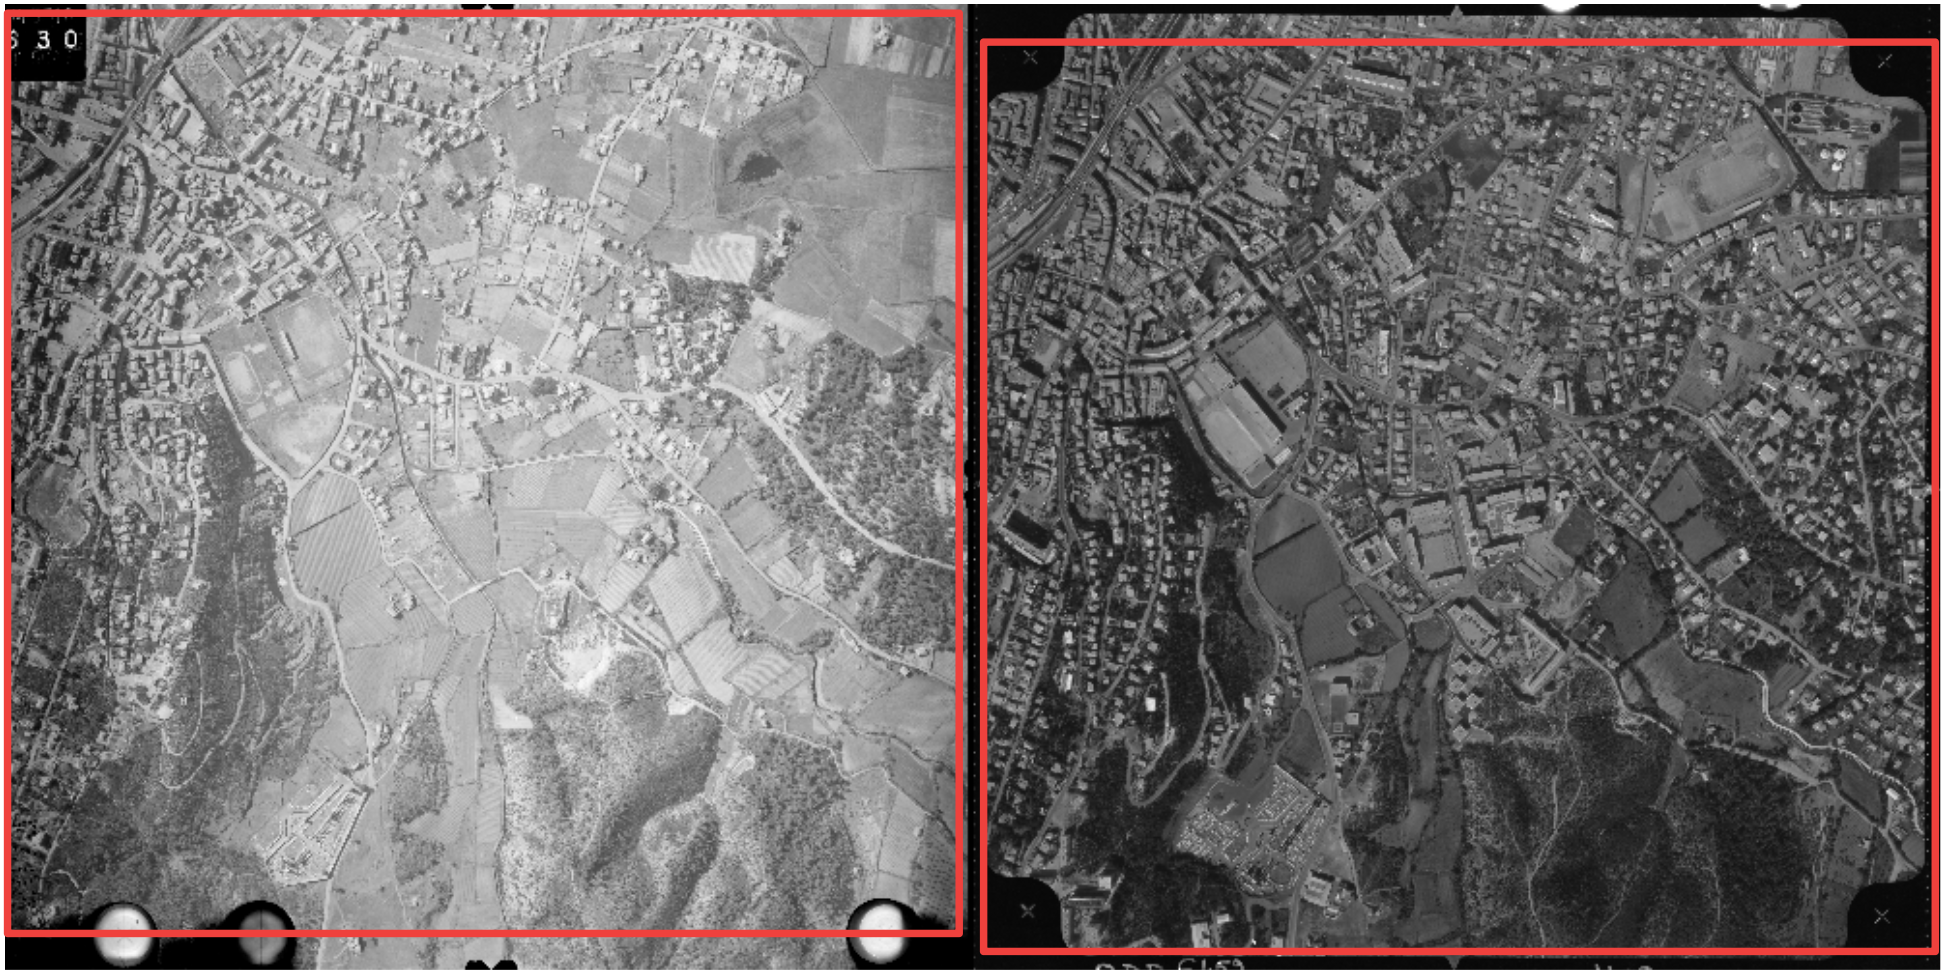
\includegraphics[width=6.2cm]{images/Chapitre1/OIS-Reech_IGNF_PVA_1-0__1954-03-06__C3544-0211_1954_CDP866_0630_OIS-Reech_IGNF_PVA_1-0__1970__C3544-0221_1970_CDP6452_1409.png}
			\end{minipage}%
		}
		\subfigure[Résultat de SIFT (0 correspondances)]{
			\begin{minipage}[t]{0.45\linewidth}
				\centering
				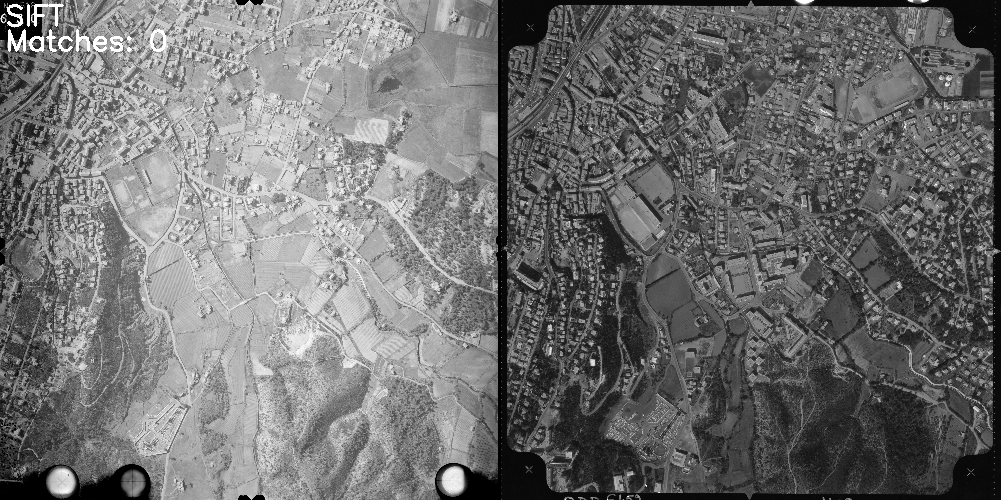
\includegraphics[width=6.2cm]{images/Chapitre1/Homol-SIFT_OIS-Reech_IGNF_PVA_1-0__1954-03-06__C3544-0211_1954_CDP866_0630_OIS-Reech_IGNF_PVA_1-0__1970__C3544-0221_1970_CDP6452_1409.png}
			\end{minipage}%
		}
		\subfigure[Résultat de SuperGlue]{
			\begin{minipage}[t]{0.45\linewidth}
				\centering
				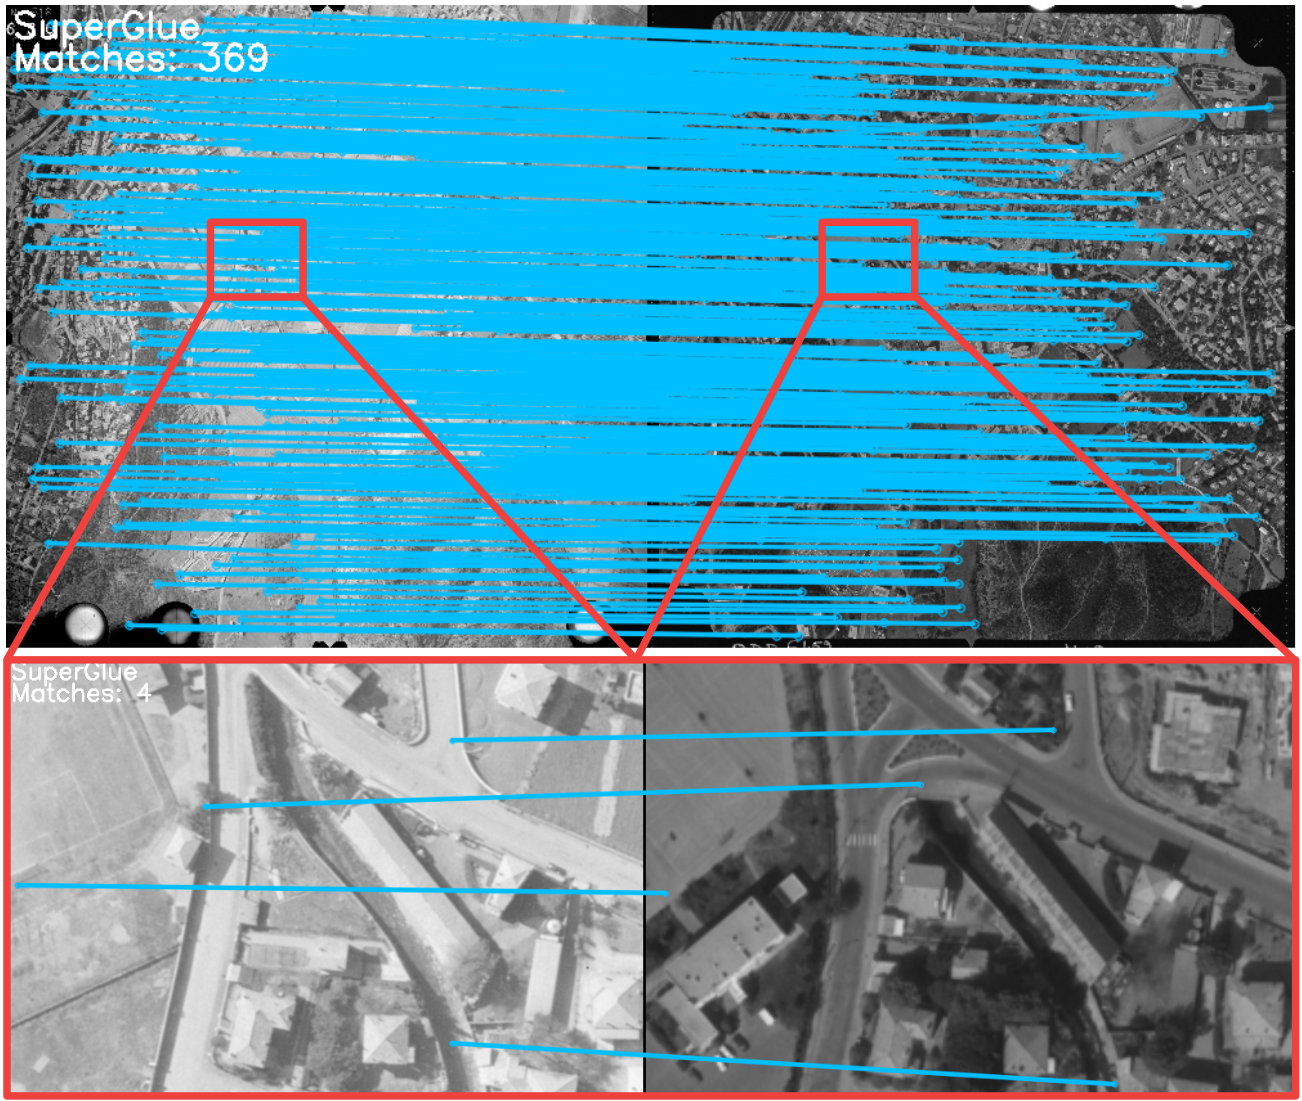
\includegraphics[width=6.2cm]{images/Chapitre1/Homol-SuperGlue_OIS-Reech_IGNF_PVA_1-0__1954-03-06__C3544-0211_1954_CDP866_0630_OIS-Reech_IGNF_PVA_1-0__1970__C3544-0221_1970_CDP6452_1409.png}
			\end{minipage}%
		}
		\subfigure[Résultat du nôtre]{
			\begin{minipage}[t]{0.45\linewidth}
				\centering
				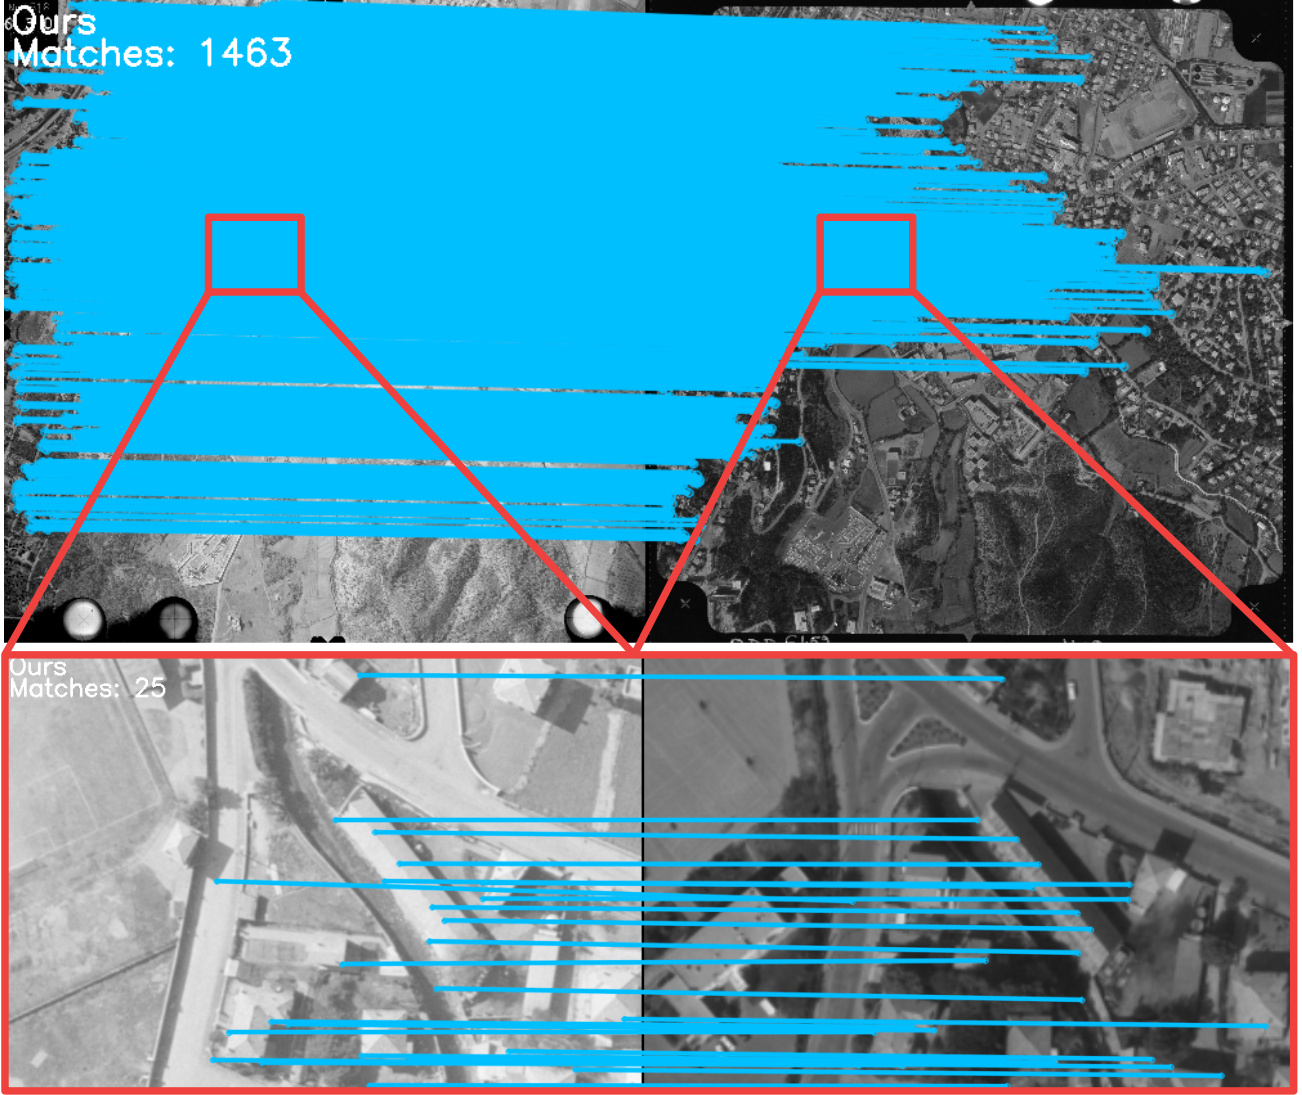
\includegraphics[width=6.2cm]{images/Chapitre1/Homol-Ours_OIS-Reech_IGNF_PVA_1-0__1954-03-06__C3544-0211_1954_CDP866_0630_OIS-Reech_IGNF_PVA_1-0__1970__C3544-0221_1970_CDP6452_1409.png}
			\end{minipage}%
		}
		\caption{(a) Une paire d'images multi-époques avec des rectangles rouges indiquant la zone de chevauchement. (b-d) Résultat de la correspondance de SIFT, SuperGlue et le nôtre.}
		\label{MultiEpoqueImgPaire}
	\end{center}
\end{figure*}

\paragraph{Avantages de la géométrie 3D}
Les images RGB sont largement utilisées pour pour l'appariement des images. Cependant, elles présentent les inconvénients suivants:\\
(1) Leur apparence change avec le temps (voir la Figure~\ref{Changementdapparence}), et avec des angles de vue variables sur des surfaces non-Lambertiennes (voir la Figure~\ref{Pauvrementtexture}).
(2) Les autosimilitudes (par exemple, les modèles répétitifs) favorisent les fausses correspondances (voir la Figure~\ref{Pauvrementtexture}).\\
Heureusement, la géométrie 3D telle que \ac{DSM} compense parfaitement ces défauts. Comme on peut le voir sur la Figure~\ref{Changementdapparence}, les images RGB sont très différentes car la scène a beaucoup changé. Cependant, les \ac{DSM} correspondants sont similaires, ce qui est raisonnable, car le paysage 3D est plus stable dans le temps. De plus, les \ac{DSM} sont plus distinctifs que les images RGB lorsqu'il s'agit de surfaces non-Lambertiennes et de motifs répétitifs, comme indiqué dans la Figure~\ref{Pauvrementtexture}. 
Même si la géométrie 3D manque de textures et de détails par rapport à l'image RGB, elle sert de complément idéal. En outre, elle joue un rôle important en fournissant des informations 3D pour établir un modèle de transformation de Helmert 3D entre les époques afin (1) de déplacer différentes époques dans le même cadre de coordonnées et (2) de supprimer les fausses correspondances dans une routine RANSAC qui est plus fiable que les modèles de transformation 2D.

\begin{figure*}[htbp]
	\begin{center}
		\subfigure[Image RGB 1971]{
			\begin{minipage}[t]{0.45\linewidth}
				\centering
				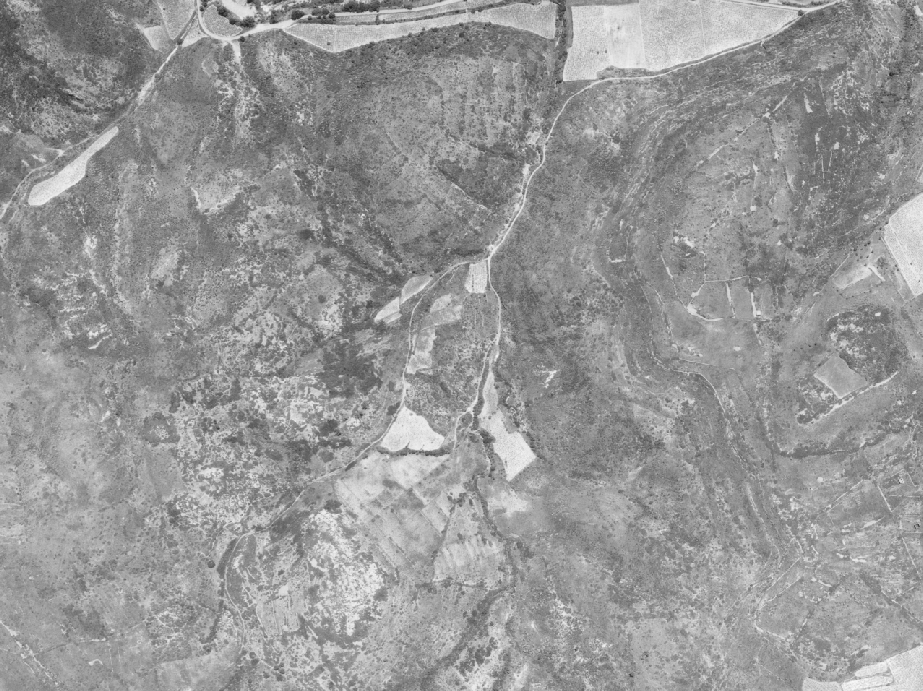
\includegraphics[width=6.2cm]{images/Chapitre1/AppearanceChangeRGBL.png}
			\end{minipage}%
		}
		\subfigure[Image RGB 2015]{
			\begin{minipage}[t]{0.45\linewidth}
				\centering
				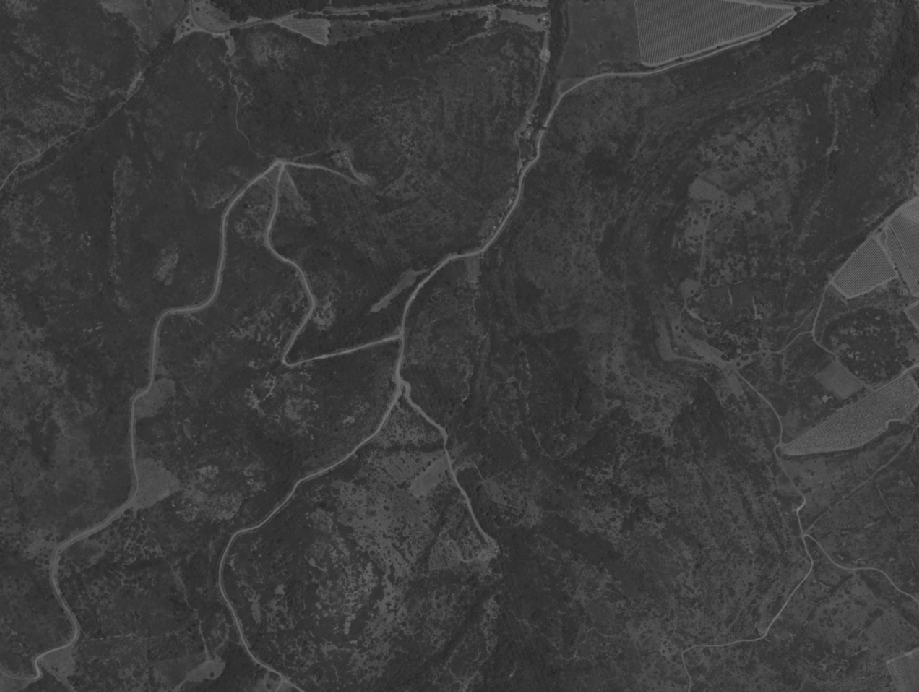
\includegraphics[width=6.2cm]{images/Chapitre1/AppearanceChangeRGBR.png}
			\end{minipage}%
		}
		\subfigure[\ac{DSM} 1971]{
			\begin{minipage}[t]{0.45\linewidth}
				\centering
				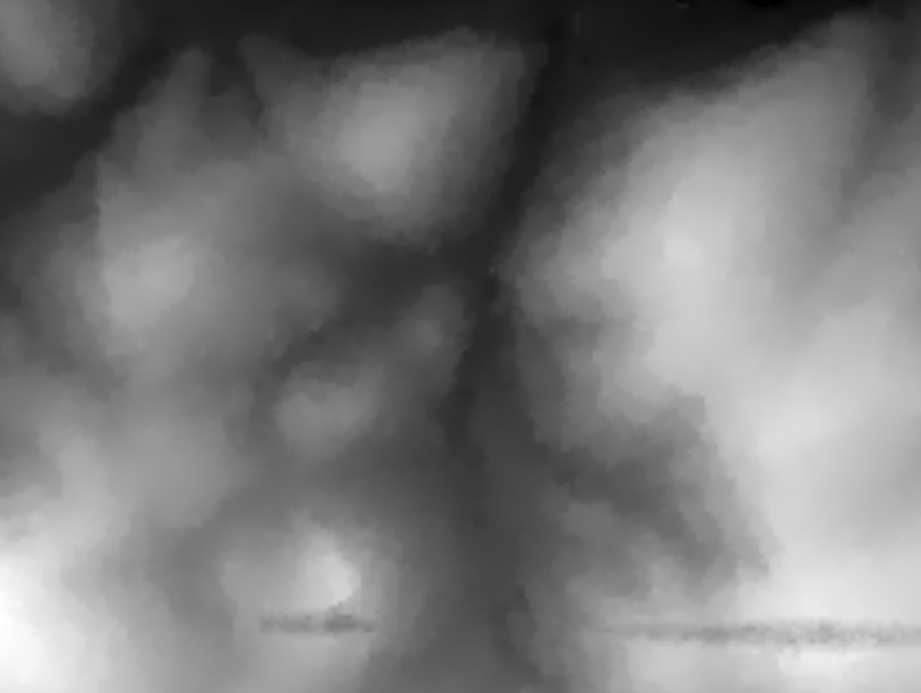
\includegraphics[width=6.2cm]{images/Chapitre1/AppearanceChangeDSML.png}
			\end{minipage}%
		}
		\subfigure[\ac{DSM} 2015]{
			\begin{minipage}[t]{0.45\linewidth}
				\centering
				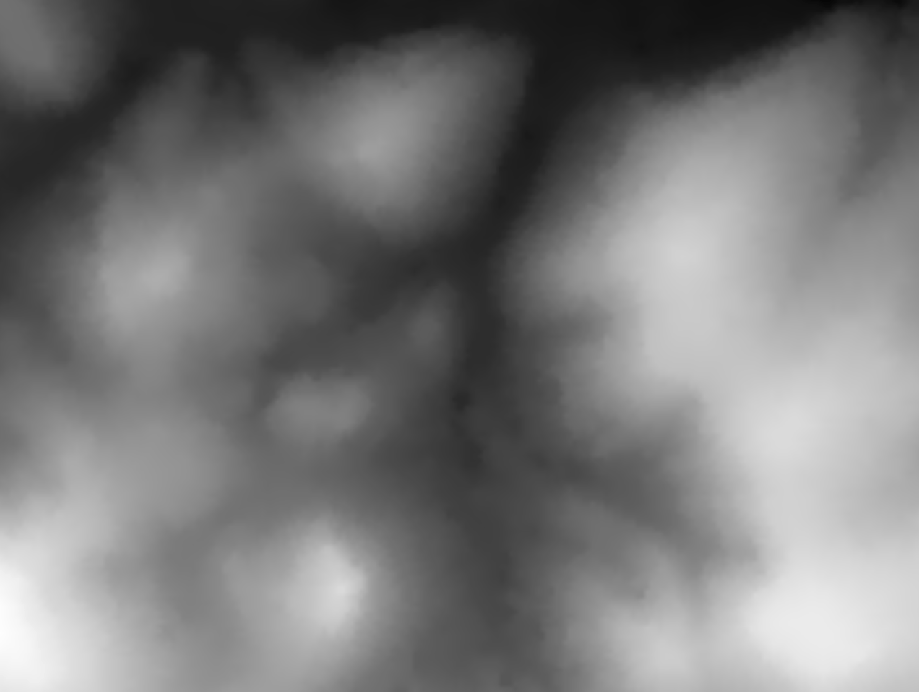
\includegraphics[width=6.2cm]{images/Chapitre1/AppearanceChangeDSMR.png}
			\end{minipage}%
		}
		\caption{La même zone observée à différents moments. Les images RGB ont beaucoup changé alors que les \ac{DSM}s sont restés stables au fil du temps.}
		\label{Changementdapparence}
	\end{center}
\end{figure*} 


\begin{figure*}[htbp]
	\begin{center}
		\subfigure[Image RGB 1971]{
			\begin{minipage}[t]{0.45\linewidth}
				\centering
				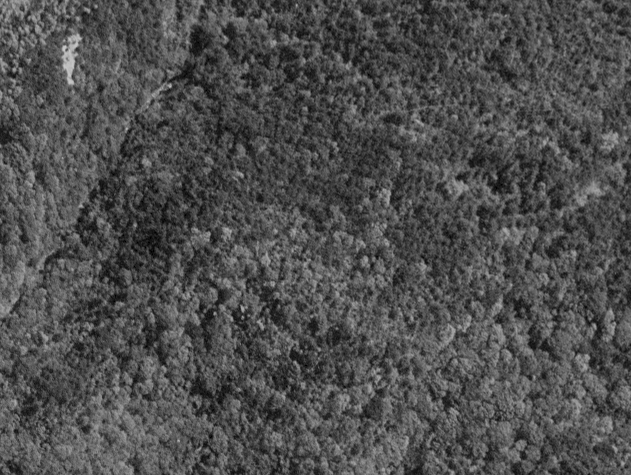
\includegraphics[width=6.2cm]{images/Chapitre1/PoorlyTexturedRGBL.png}
			\end{minipage}%
		}
		\subfigure[Image RGB 2015]{
			\begin{minipage}[t]{0.45\linewidth}
				\centering
				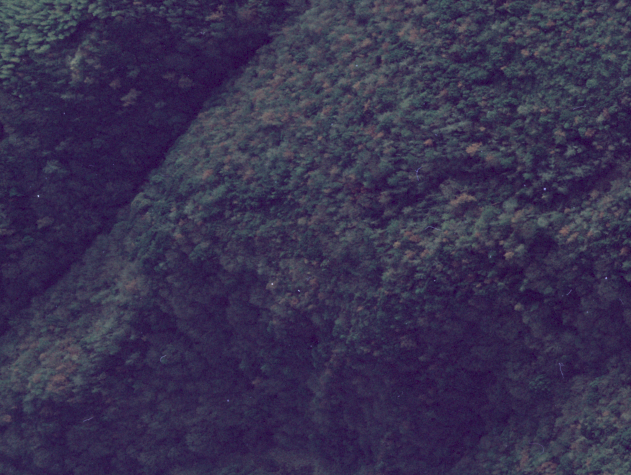
\includegraphics[width=6.2cm]{images/Chapitre1/PoorlyTexturedRGBR.png}
			\end{minipage}%
		}
		\subfigure[\ac{DSM} 1971]{
			\begin{minipage}[t]{0.45\linewidth}
				\centering
				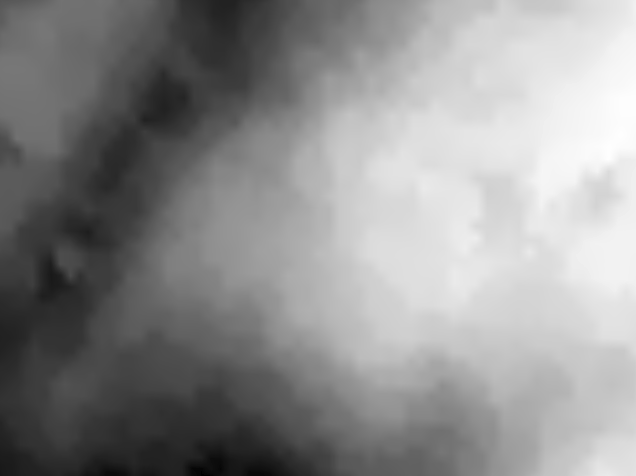
\includegraphics[width=6.2cm]{images/Chapitre1/PoorlyTexturedDSML.png}
			\end{minipage}%
		}
		\subfigure[\ac{DSM} 2015]{
			\begin{minipage}[t]{0.45\linewidth}
				\centering
				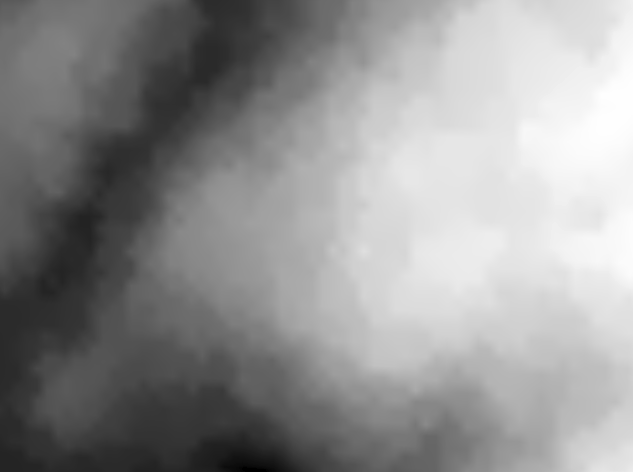
\includegraphics[width=6.2cm]{images/Chapitre1/PoorlyTexturedDSMR.png}
			\end{minipage}%
		}
		\caption{La même végétation observée à des moments différents. Réflexion non-lambertienne et autosimilitude présentes dans les images RGB, tandis que les \ac{DSM}s restent distinctifs.}
		\label{Pauvrementtexture}
	\end{center}
\end{figure*} 

\paragraph{Diviser et conquérir}
Puisque la récupération de correspondances robustes et précises sur des paires d'images multi-époques est une tâche difficile, nous divisons la tâche en deux sous-tâches et les conquérons individuellement avec la stratégie grossier-à-précis. Cette stratégie est illustrée dans la Figure~\ref{grossier-à-précis}. Les deux sous-tâches sont les suivantes:\\
\begin{enumerate}
	\item Co-enregistrement grossier, comme illustré sur la Figure~\ref{grossier-à-précis}(b). Son objectif est d'aligner grossièrement les paires d'images multi-époques en se concentrant sur la robustesse et en relâchant l'exigence de précision.
	\item Appariement précis, comme illustré sur la Figure~\ref{grossier-à-précis}(c). Elle améliore les correspondances prédites par le résultat grossier du co-enregistrement en recherchant uniquement le voisinage local pour réduire l'ambiguïté.
\end{enumerate}
\begin{figure*}[htbp]
	\begin{center}
		\subfigure[Exemple d'une paire d'images inter-époques]{
			\begin{minipage}[t]{1\linewidth}
				\centering
				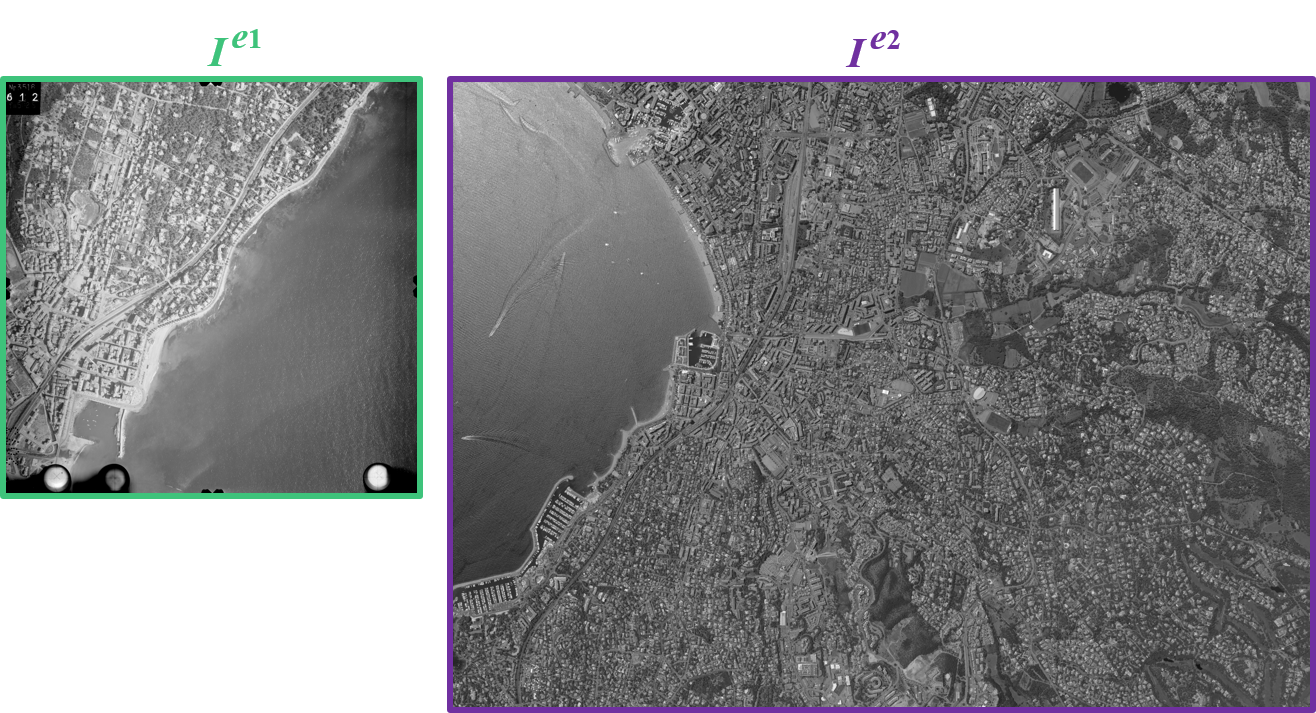
\includegraphics[width=1\columnwidth]{images/Chapitre1/imagepair.png}
			\end{minipage}%
		}
		\subfigure[Co-enregistrement grossier]{
			\begin{minipage}[t]{1\linewidth}
				\centering
				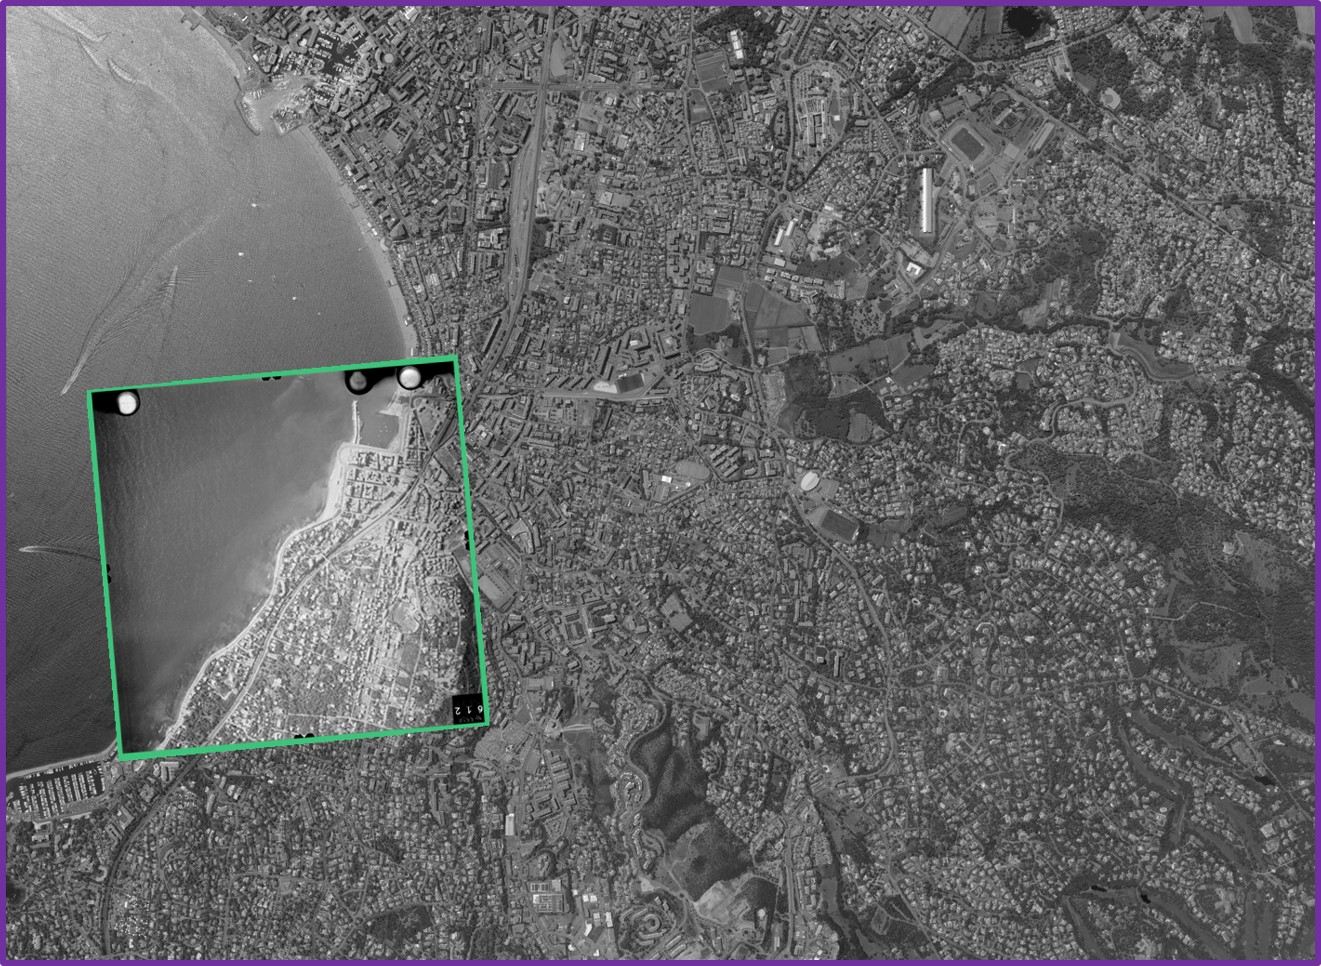
\includegraphics[width=0.68\columnwidth]{images/Chapitre1/CoReg.jpg}
			\end{minipage}%
		}
		\subfigure[Appariement précis]{
			\begin{minipage}[t]{1\linewidth}
				\centering
				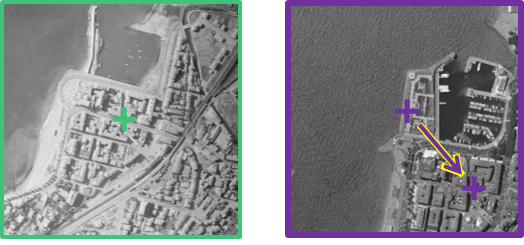
\includegraphics[width=0.55\columnwidth]{images/Chapitre1/Precise.png}
			\end{minipage}%
		}
		\caption{Stratégie grossier-à-précis. (a) Un exemple de paire d'images inter-époques à apparier. $I^{e_1}$ et $I^{e_2}$ représentent les images prises à $epoch_1$ et $epoch_2$ individuellement. (b) Illustration du co-enregistrement grossier entre $I^{e_1}$ et $I^{e_2}$. En conséquence, $I^{e_1}$ est grossièrement aligné avec $I^{e_2}$. (c) Illustration de l'appariement précis. Pour les points clés de $I^{e_1}$ (croix verte), un emplacement est prédit dans $I^{e_2}$ (croix violette) sur la base d'un co-enregistrement grossier, dont le voisinage local sera recherché pour trouver l'appariement précis (croix jaune).}
		\label{grossier-à-précis}
	\end{center}
\end{figure*}

\section{Contributions}
Dans cette thèse, nous présentons des pipelines grossiers-à-précis pour l'appariement d'images multi-époques. Ils sont adaptés aux images aériennes, satellitaires et mixtes, ce qui ouvre la possibilité de géoréférencer des millions d'images historiques sans nécessiter de \ac{GCP}s. 
Six variantes sont proposées pour l'étape de co-enregistrement grossier et deux variantes pour l'étape d'appariement précis. Chaque variante a sa propre caractéristique:\\
\begin{enumerate}
	\item Pour les variantes de co-enregistrement grossier: (1) celles basées sur l'idée d'appariement des \ac{DSM}s conduisent généralement aux résultats les plus robustes ; (2) celles qui apparient les orthophotos pourraient servir d'alternatives dans les rares scénarios de terrain parfaitement plat où les \ac{DSM}s ne fournissent pas d'informations utiles ; (3) les autres qui apparient les paires d'images originales conduisent souvent à des résultats moins satisfaisants, mais ce sont les seules options adaptées aux images terrestres.
	\item Pour les variantes d'appariement précis: (1) $Patch$ est basé sur des méthodes d'appariement par apprentissage, il donne généralement plus de correspondances car il est plus invariant dans le temps. (2) $Guided$ est basé sur des méthodes artisanales, il est plus efficace en termes d'utilisation de la mémoire et des ressources CPU car il n'implique pas de rééchantillonnage des patchs, ce qui est nécessaire pour $Patch$. 
\end{enumerate}
\par
Nos pipelines visent à libérer le potentiel des images historiques pour le suivi des conditions environnementales. 
Nous collaborons actuellement avec plusieurs instituts pour appliquer nos pipelines dans différentes applications, notamment:\\
\begin{enumerate}
	\item Institut de Physique du Globe de Paris (IPGP) et Korea Institute of Geoscience and Mineral Resources (KIGAM) pour analyser les déformations de la croûte terrestre afin de comprendre les événements sismiques.
	\item Conseil national de la recherche, Institut de recherche pour la protection hydrogéologique (CNR-IRPI) pour l'analyse de l'évolution des glissements de terrain en Italie.
	\item Département des sciences de la terre et de l'environnement de l'université de Pavie pour l'analyse de l'évolution des badlands en Europe.
\end{enumerate}
\par
Nous avons également développé deux tutoriels complets accompagnés d'ensembles de données de test pour familiariser les utilisateurs avec nos pipelines implémentés dans MicMac\cite{HistoPcode} (plus de détails sont présentés dans l'annexe \ref{chap:appendixC}):\\
\begin{enumerate}
	\item Tutoriel d'appariement des images aériennes \cite{tuto-aerial} 
	\item Tutoriel d'appariement d'images mixtes (c'est-à-dire d'images aériennes et satellitaires) \cite{tuto-mixed} 
\end{enumerate}
\par
Publications de l'auteur:\\
\begin{enumerate}
	\item M Santangelo, \textbf{L Zhang}, E Rupnik, M Pierrot-Deseilligny, M Cardinali. Schéma d'évolution des glissements de terrain révélé par des MNS multitemporels obtenus à partir d'images aériennes historiques. ISPRS Archives of the Photogrammetry, Remote Sensing and Spatial Information Sciences, 2022.
	\item \textbf{L Zhang}, E Rupnik, M Pierrot-Deseilligny. Appariement des caractéristiques pour des images aériennes historiques multi-époques, 182, 176-189, 2021.
	\item \textbf{L Zhang}, E Rupnik, M Pierrot-Deseilligny. Appariement des caractéristiques guidé pour l'estimation de la pose de blocs d'images historiques multi-époques. ISPRS Annals of the Photogrammetry, Remote Sensing and Spatial Information Sciences, 2020.
\end{enumerate}
Nous fournissons également une vidéo \cite{HistoPVideo}, des diapositives \cite{HistoPSlides} et le site web du projet \cite{HistoPProj} pour améliorer la visibilité de notre travail.\\

\section{Organisation de la thèse}
Cette thèse présente des pipelines entièrement automatiques pour l'appariement d'images multi-époques. 
Une brève présentation de \textit{l'état de l'art} est donnée dans le \textbf{Chapitre}~\ref{chap:review}.\\

Dans le \textbf{Chapitre}~\ref{chap:ApplicationsAndDatasets}, les applications ainsi que 5 données représentatifs sont présentés, qui sont ensuite utilisés pour tester nos pipelines.\\

Dans le \textbf{Chapitre}~\ref{chap:RoughCoReg}, six variantes de co-enregistrement grossier sont élaborées pour aligner grossièrement le bloc entier en construisant un modèle de transformation globalement cohérent entre les époques différentes.\\

Dans le \textbf{Chapitre}~\ref{chap:Precisematching}, deux variantes d'appariement précis sont introduites pour obtenir des appariements exacts sous la direction des orientations et des \ac{DSM} qui sont grossièrement co-registrés.\\

Enfin, le \textbf{Chapitre} ~\ref{chap:conclusion} présente les conclusions et les perspectives.\\
